\chapter{Background}

In this chapter, an introduction to the various research areas which
have heavily influenced this thesis is provided.

% \section{Problem Definition}

% \section{Notation (Not sure if this is necessary yet)}



\section{Neural Networks}


\subsection{Gradient Descent}

Neural networks have significantly grown in size since their
inception. A neural network model of today may contain as many as
fifty million parameters. This establishes a difficult, extremely
large, non-convex optimisation problem. The only way to sensibly train
these models, ignoring minor implementation details, is to use
gradient descent optimisation.


To assist in the explanation of gradient descent, suppose a
classification problem with annotated training data
$Z = \{(x_i, y_i)\}$, containing images $x_i$ each with a
corresponding label $y_i$. We define $f$ as the classifier, mapping
image $x_i$ to label $y_i$ given a real vector of parameters $\theta$,
\begin{equation}
  y_i \approx f(x_i;\theta) .
\end{equation}

\noindent To measure the performance this classifier, a loss function
$\ell$ is defined, which is entirely dependant on the problem at hand,

\begin{equation}
  loss = \sum_i \ell(y_i, f(x_i ; \theta) .
\end{equation}


\noindent Initially parameters $\theta$ will be unknown. Hence, in
order to find $\theta$ (so that we can establish a trained
classifier), we must minimise the loss function,
\begin{equation}
  \min_\theta \sum_i \ell(y_i, f(x_i ; \theta)) .
\end{equation}



\noindent This minimisation is typically performed using gradient
descent, where $\theta$ is gradually learnt over many iterations. This
is at rate $\eta$ (known as the \textit{learning rate}), and is
directed by the gradient of the $f$ with parameters $\theta$,

\begin{equation}
  \theta = \theta - \eta \nabla_\theta \ell(y_i, f(x_i ; \theta) .
  \end{equation}

More often than not, the above is extended to support batches of
images per iteration. This is referred to as Minibatch Gradient
Descent and results in more a stable gradient due to the averaging
across several images. An additional benefit to using minibatch
gradient descent is more efficient use of resources as the training
can be parallelised.

\subsection{Convolutional Neural Networks}

In the previous subsection, an overview of gradient descent was
presented, where parameters $\theta$ were used to \textit{in some way}
to apply a mapping from image to label. Such a function might be
defined as simply as a linear function, $f(x;\theta) = \theta
x$. Unfortunately, despite being appropriate in many areas, a linear
function will struggle to map a non-linear problem, with is often the
case with computer vision based applications. As such, convolutions
are often used to both reduce the number of parameters, and to allow
convenient and efficient stacking, allowing the network to map learn
difficult mappings.

Convolutional Neural Networks (CNNs) are constructed, typically, from
stacks of convolutional filters, each followed by some form of
transfer function. The tailing end of a CNN is often specific to each
application. For example, for a numerical regression task, linear
layers may be added, and for segmentation, a $1\times 1$ convolution
may be added. As these networks have gradually increased in size, the
term \textit{Deep Learning} has become popular. Networks of today may
consist of several hundred convolutional layers, such as
ResNet-152~\cite{he2015deep}.

% \begin{tikzpicture}[scale=0.75]
%     \draw[step=0.5,gray,thin,yslant=0.4] (0.5,0.5) grid (6,6);
%     \node[above,yslant=0.4] at (3,7.2) {Input Image};
%     \draw[step=1,red,thick,yslant=0.4,fill=orange]  (4,1) grid (7,4);
%     \draw[yslant=0.4,dashed,red] (3,3.5) -- (4,4);
%     \draw[yslant=0.4,dashed,red] (3,2) -- (4,1);
%     \draw[yslant=0.4,dashed,red] (4.5,3.5) -- (7,4);
%     \draw[yslant=0.4,dashed,red] (4.5,2) -- (7,1);

%     \begin{scope}[shift={(8,0)}]
%       \draw[step=0.5,gray,thin,yslant=0.4] (0.5,0.5) grid (6,6);
%       \node[above,yslant=0.4] at (3,7.2) {Output Feature Map};
%     \end{scope}

%   \end{tikzpicture}

\subsection{Batch Normalisation}

As networks grew from 15 or so layers upwards, the job of gradient
descent became very difficult. During training, the distribution of
every input to every layer changes slightly. This is because the
parameters of the layer before each layer change. This problem is
referred to as \textit{internal covariate shift}. A solution known as
Batch Normalisation was proposed in~\cite{ioffe2015batch}, enabling
networks with many layers (such as the 152 layers in
ResNet~\cite{he2015deep}) to be trained either at all, or in much
shorter times. Some additional advantages of using batch normalisation
include being able to use larger learning rates and reducing the need
for careful initialisation.

Batch normalisation works as the name might suggest, by normalising
the output of each parameterised layer using learnable scale and shift
parameters, as well as the size of each minibatch, for each
minibatch. Understanding exactly how batch normalisation works is not
imperative to understanding the contents of this thesis. However, in
general, batch normalisation has been applied either before or after
every parameterised layer of the CNN models proposed in this
thesis. Additionally, as these networks are very large, they are
unlikely to have been possible to train without employing batch
normalisation.


\subsection{Frameworks}

While designing and developing a framework to work with deep neural
networks \textit{might} be an interesting thought experiment for some,
it is far from the focus of this thesis. The work presented throughout
this thesis was developed primarily under the
Torch~\footnote{\url{http://torch.ch/}, except for the work on facial
  part segmentation, which was developed under
  Cafe~\cite{jia2014caffe}}. There are a number of reasons for this,
but to name just a few:

\begin{enumerate}
\item Efficient GPU support. This is important, of course, in any
  framework intended for deep learning. Torch enables networks to be
  run in parallel (for speed) or sequentially (for additional memory)
  across multiple GPUs.
\item Elegant memory backend. Data can be loaded directly into memory
  and views can be applied to create $N$-dimensional Tensors without
  shuffling memory. This is very important when reading in large
  volumetric training samples.
\item Multithreading. The trade offs between I/O and CPU are discussed
  in more detail in Section~\ref{sec:background:volstorage}. However,
  regardless of how the data is optimised (in terms of compression or
  just raw data), volumes are big. Loading them sequentially and
  applying augmentation, even on very fast hardware, remains a
  computationally expensive task.
\end{enumerate}


\section{3D Volumes and Volumetric Algorithms}

Typically, 3D models are provided as a mesh, defined by vertices and
faces, in a particular file format such as \textit{Wavefront
  Obj}. These files typically contain additional data, such as texture
mapping coordinates and surface normals. To represent the structure of
an object, only the mesh is required. However, an alternative approach
to representing the structure of an object is to encode it in a three
dimensional volume. This may be thought of as a 3D matrix, where
\textit{inside} the object is denoted by a one, and \textit{outside}
is denoted with a zero.

\begin{figure}
  \begin{tabular}{ccccc}
    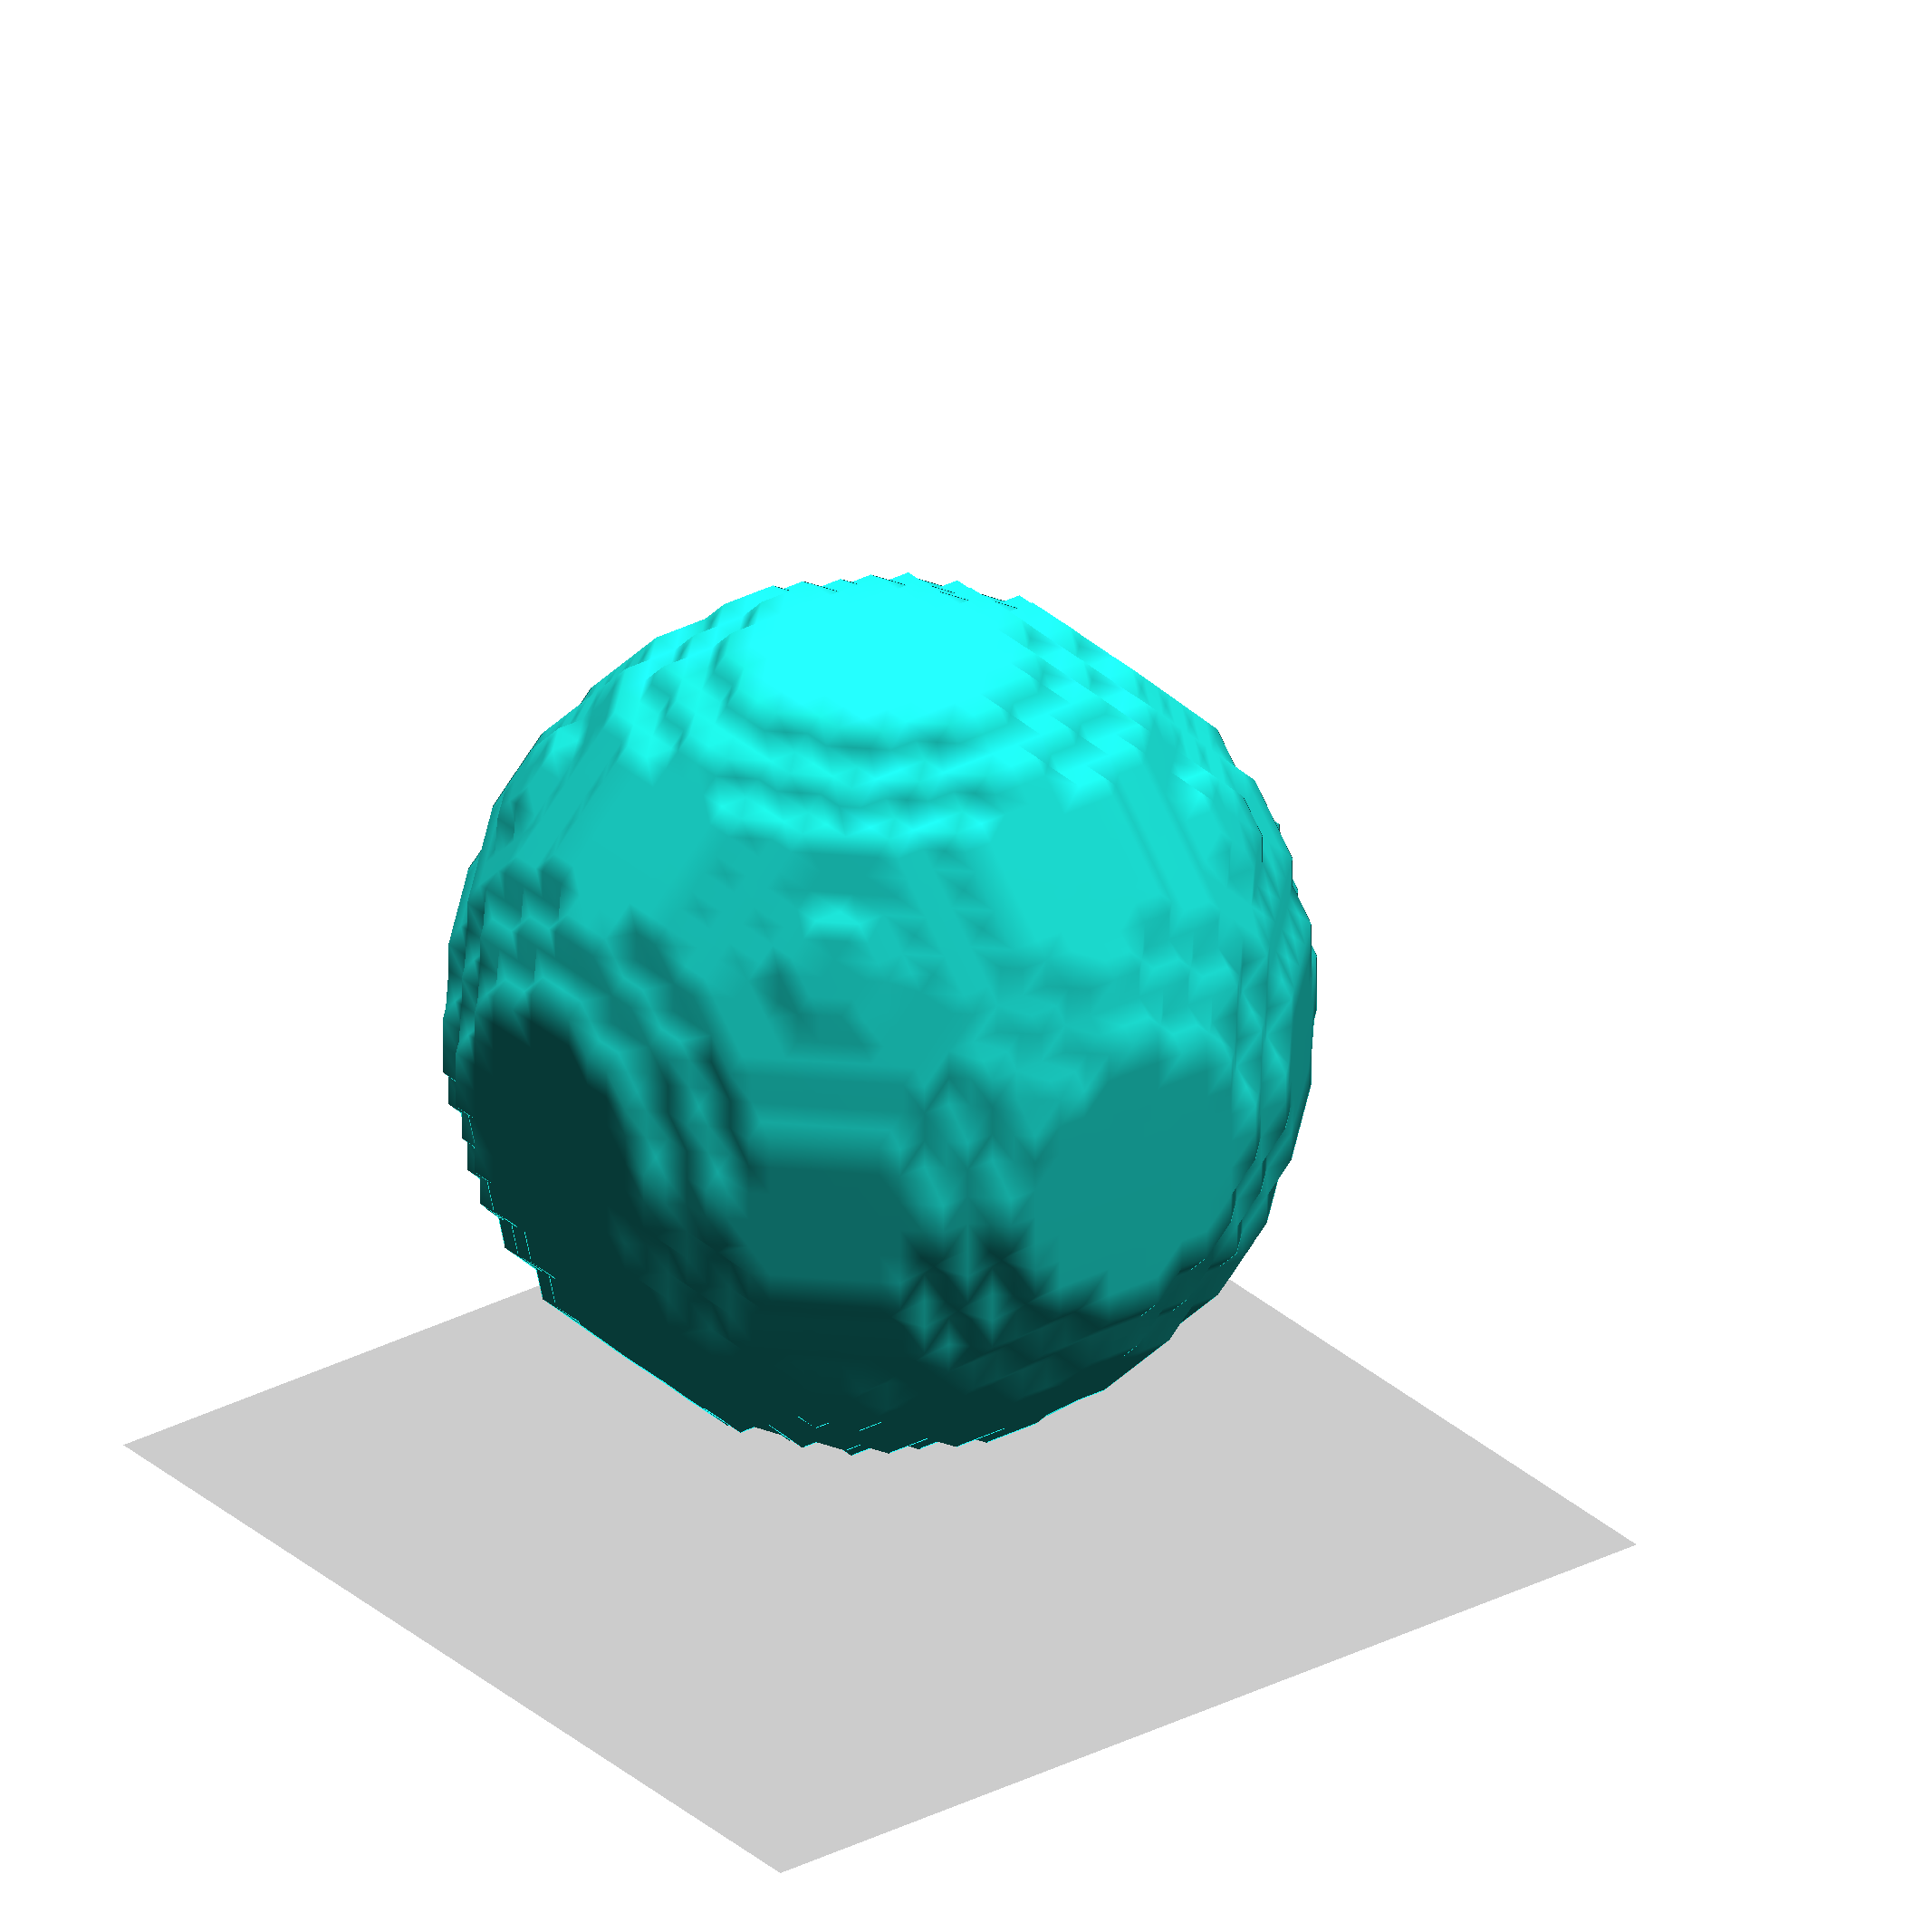
\includegraphics[width=0.18\linewidth]{chapter_background/img/binary_32x32x32.png} &
    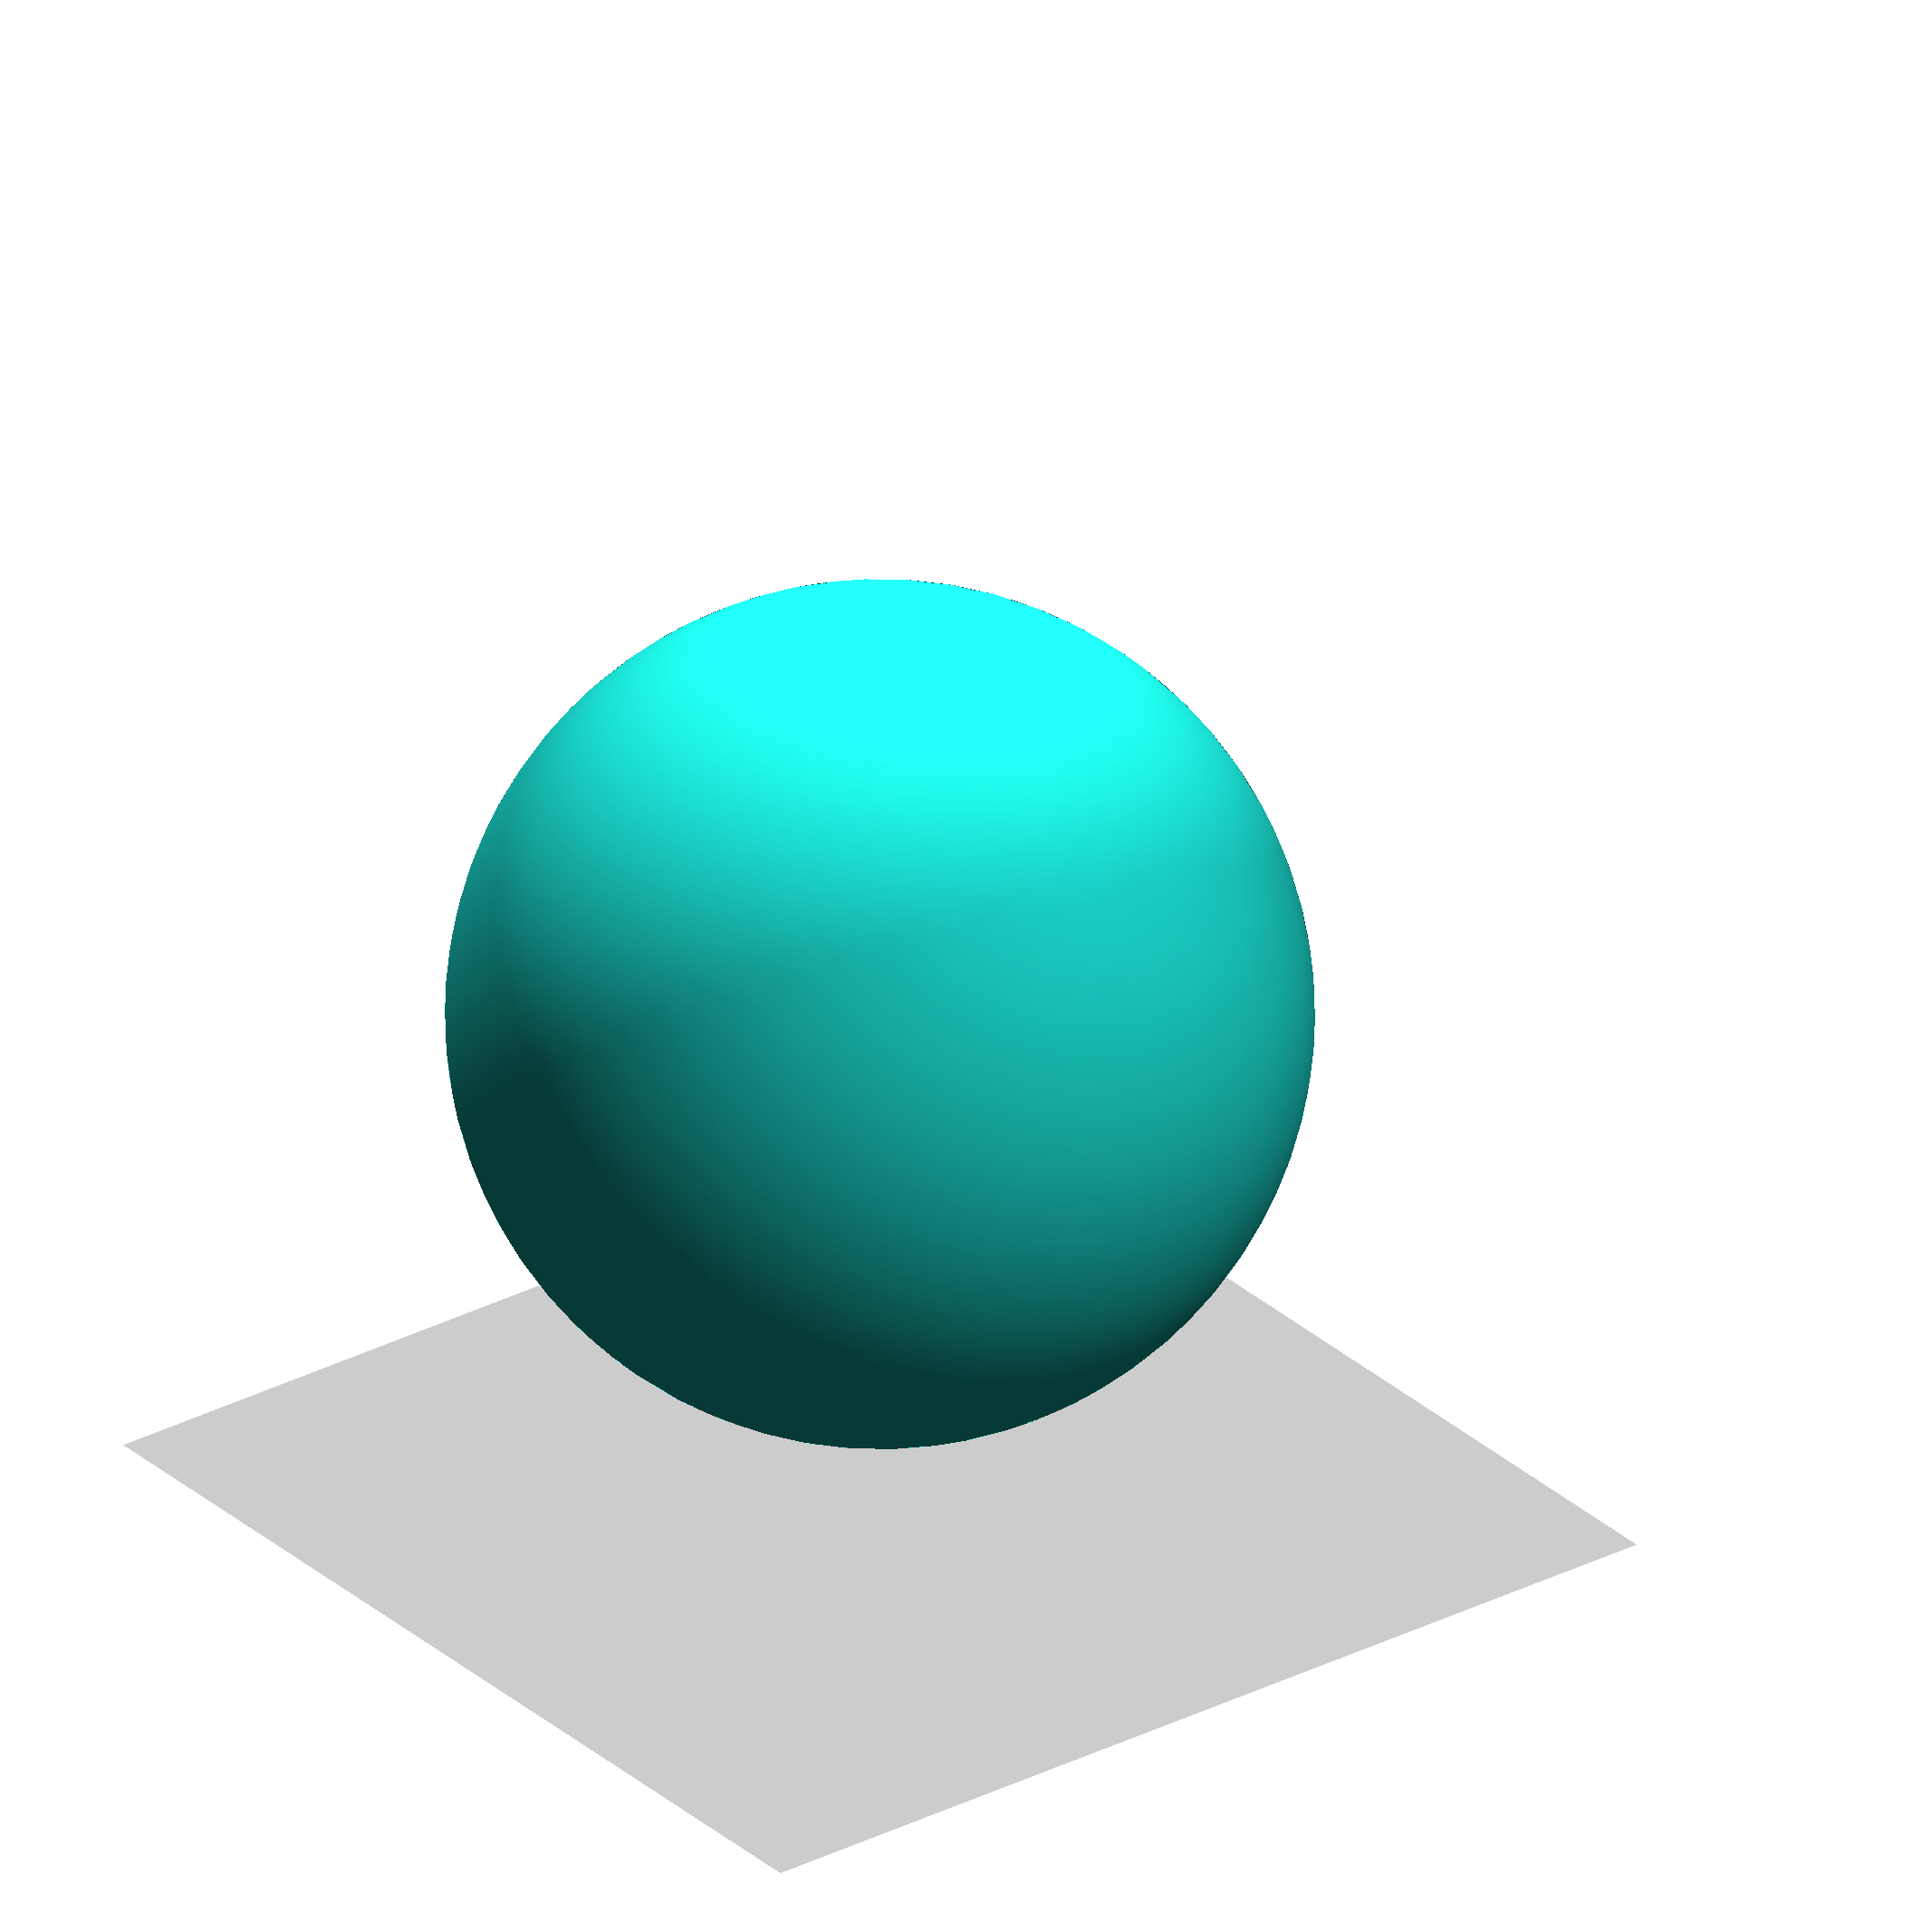
\includegraphics[width=0.18\linewidth]{chapter_background/img/real_32x32x32.png} &
    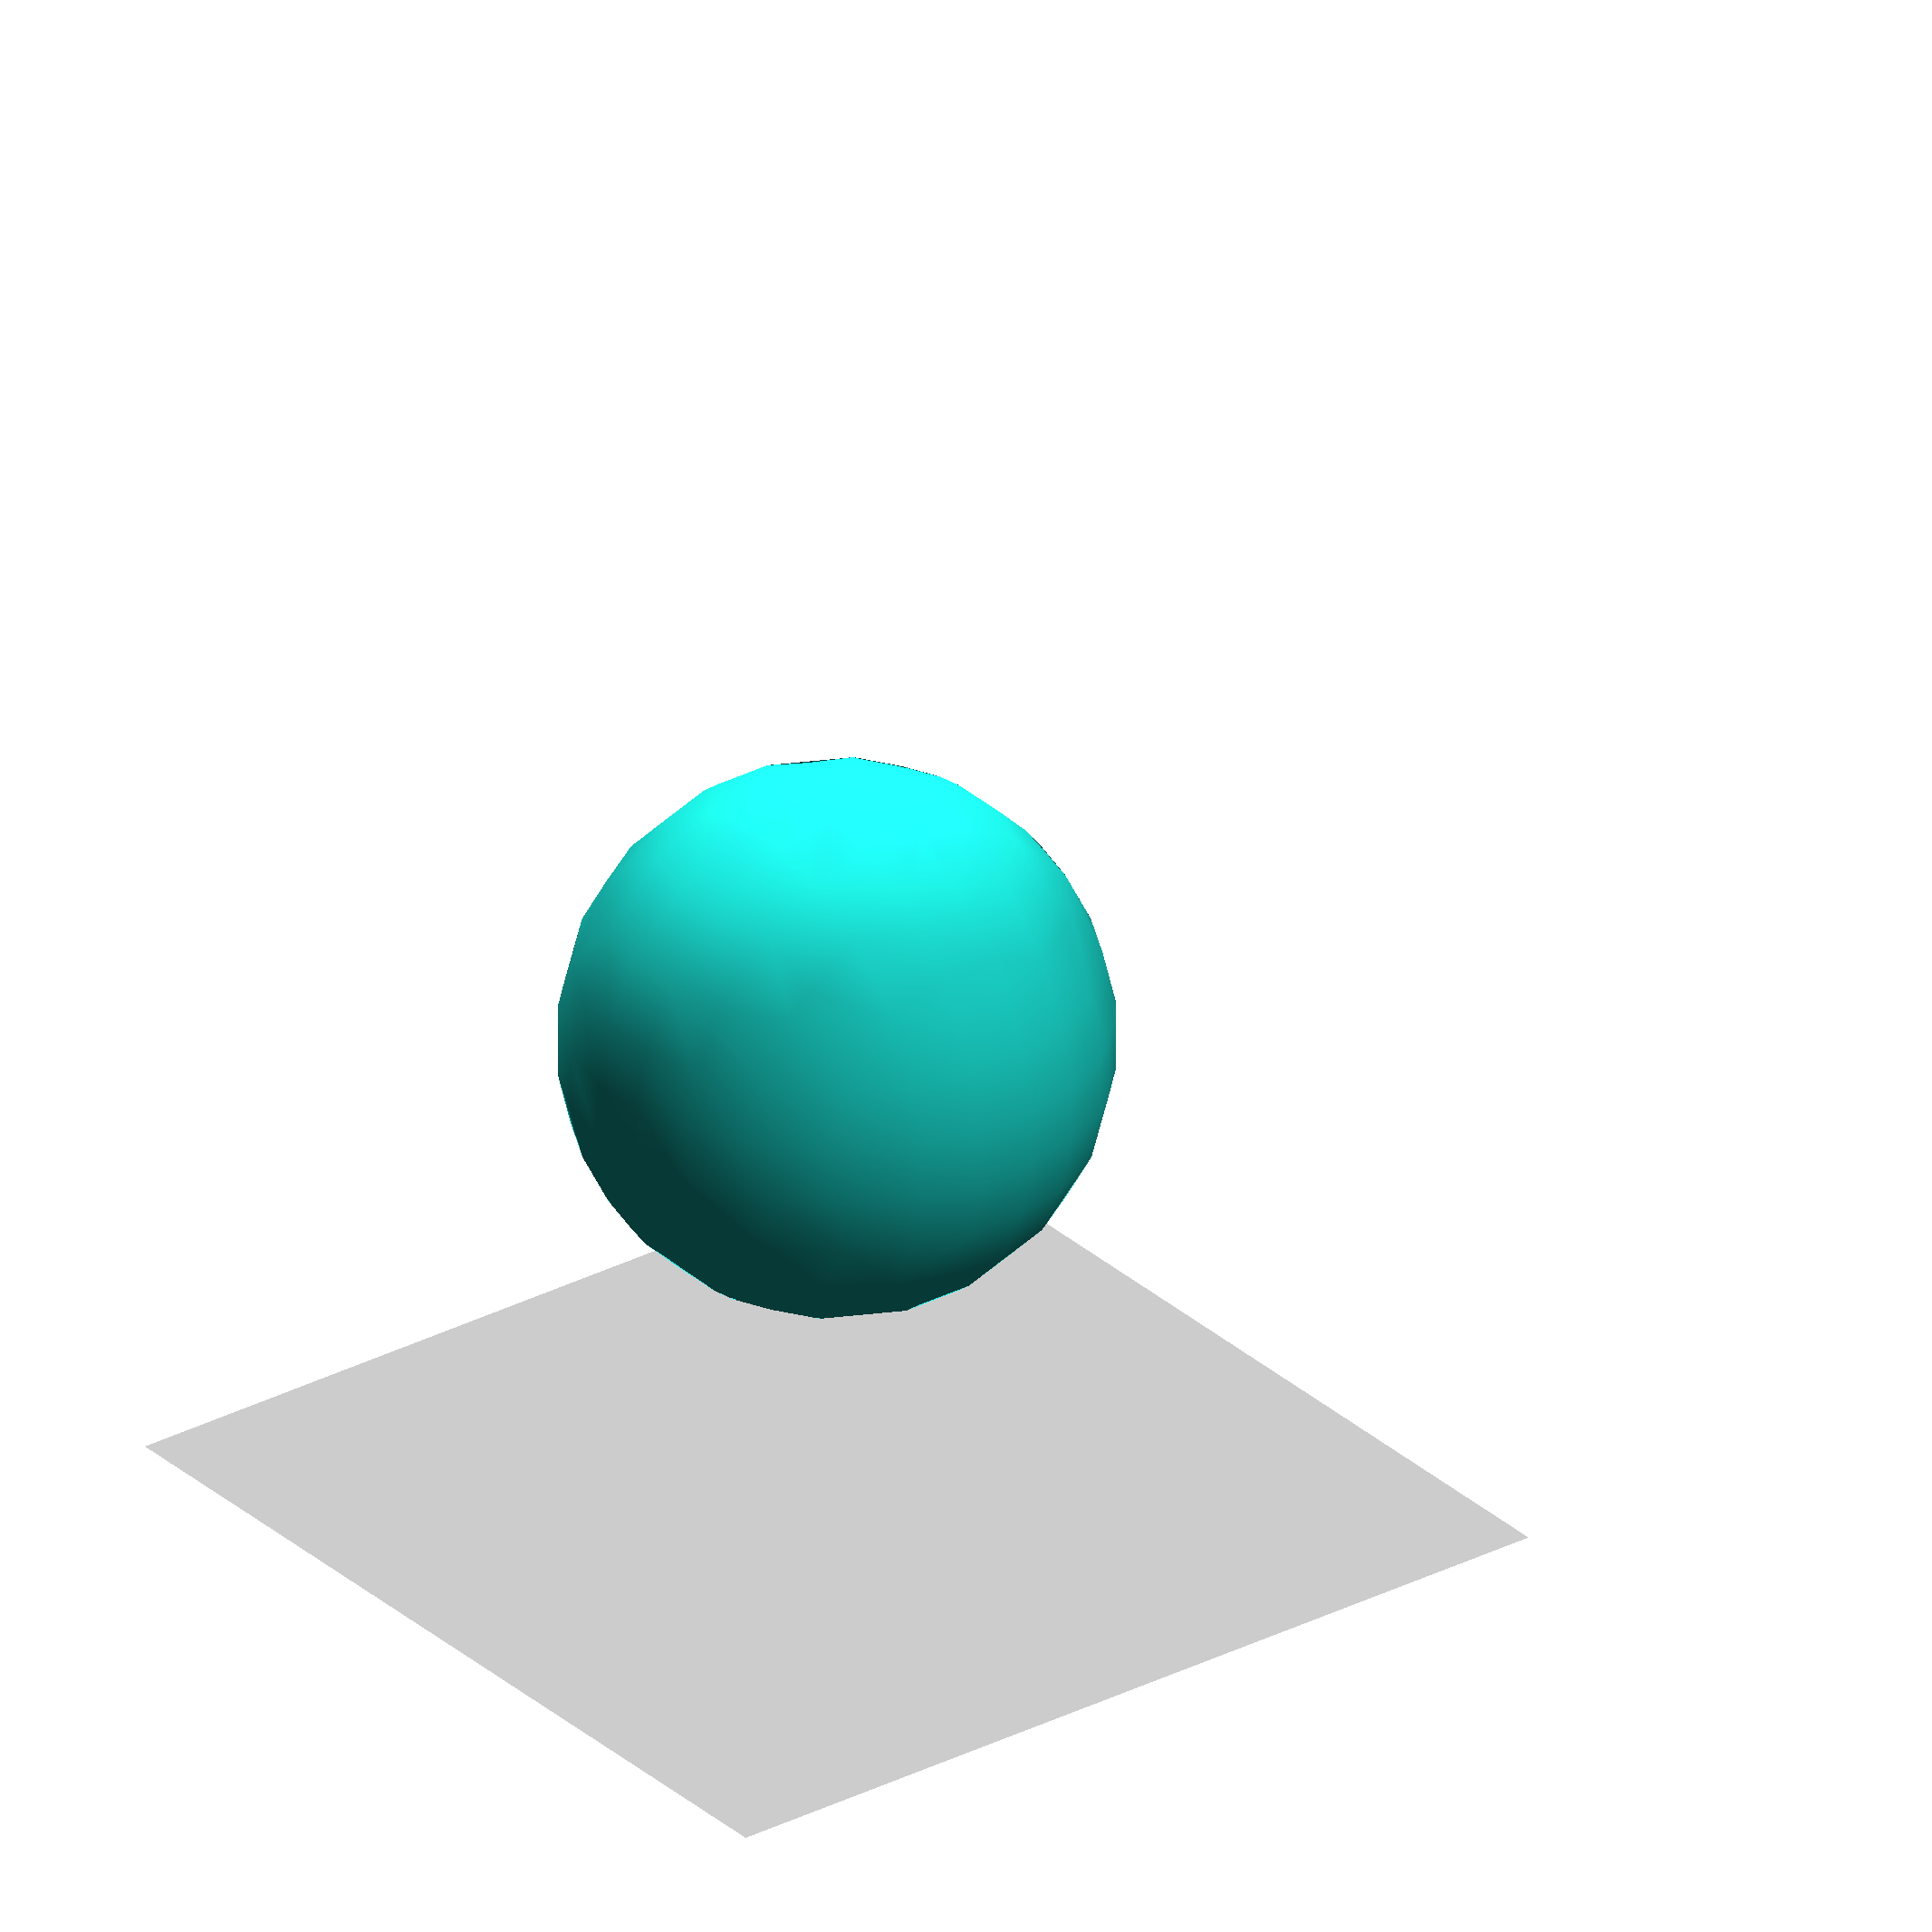
\includegraphics[width=0.18\linewidth]{chapter_background/img/real_16x16x16.png} &
    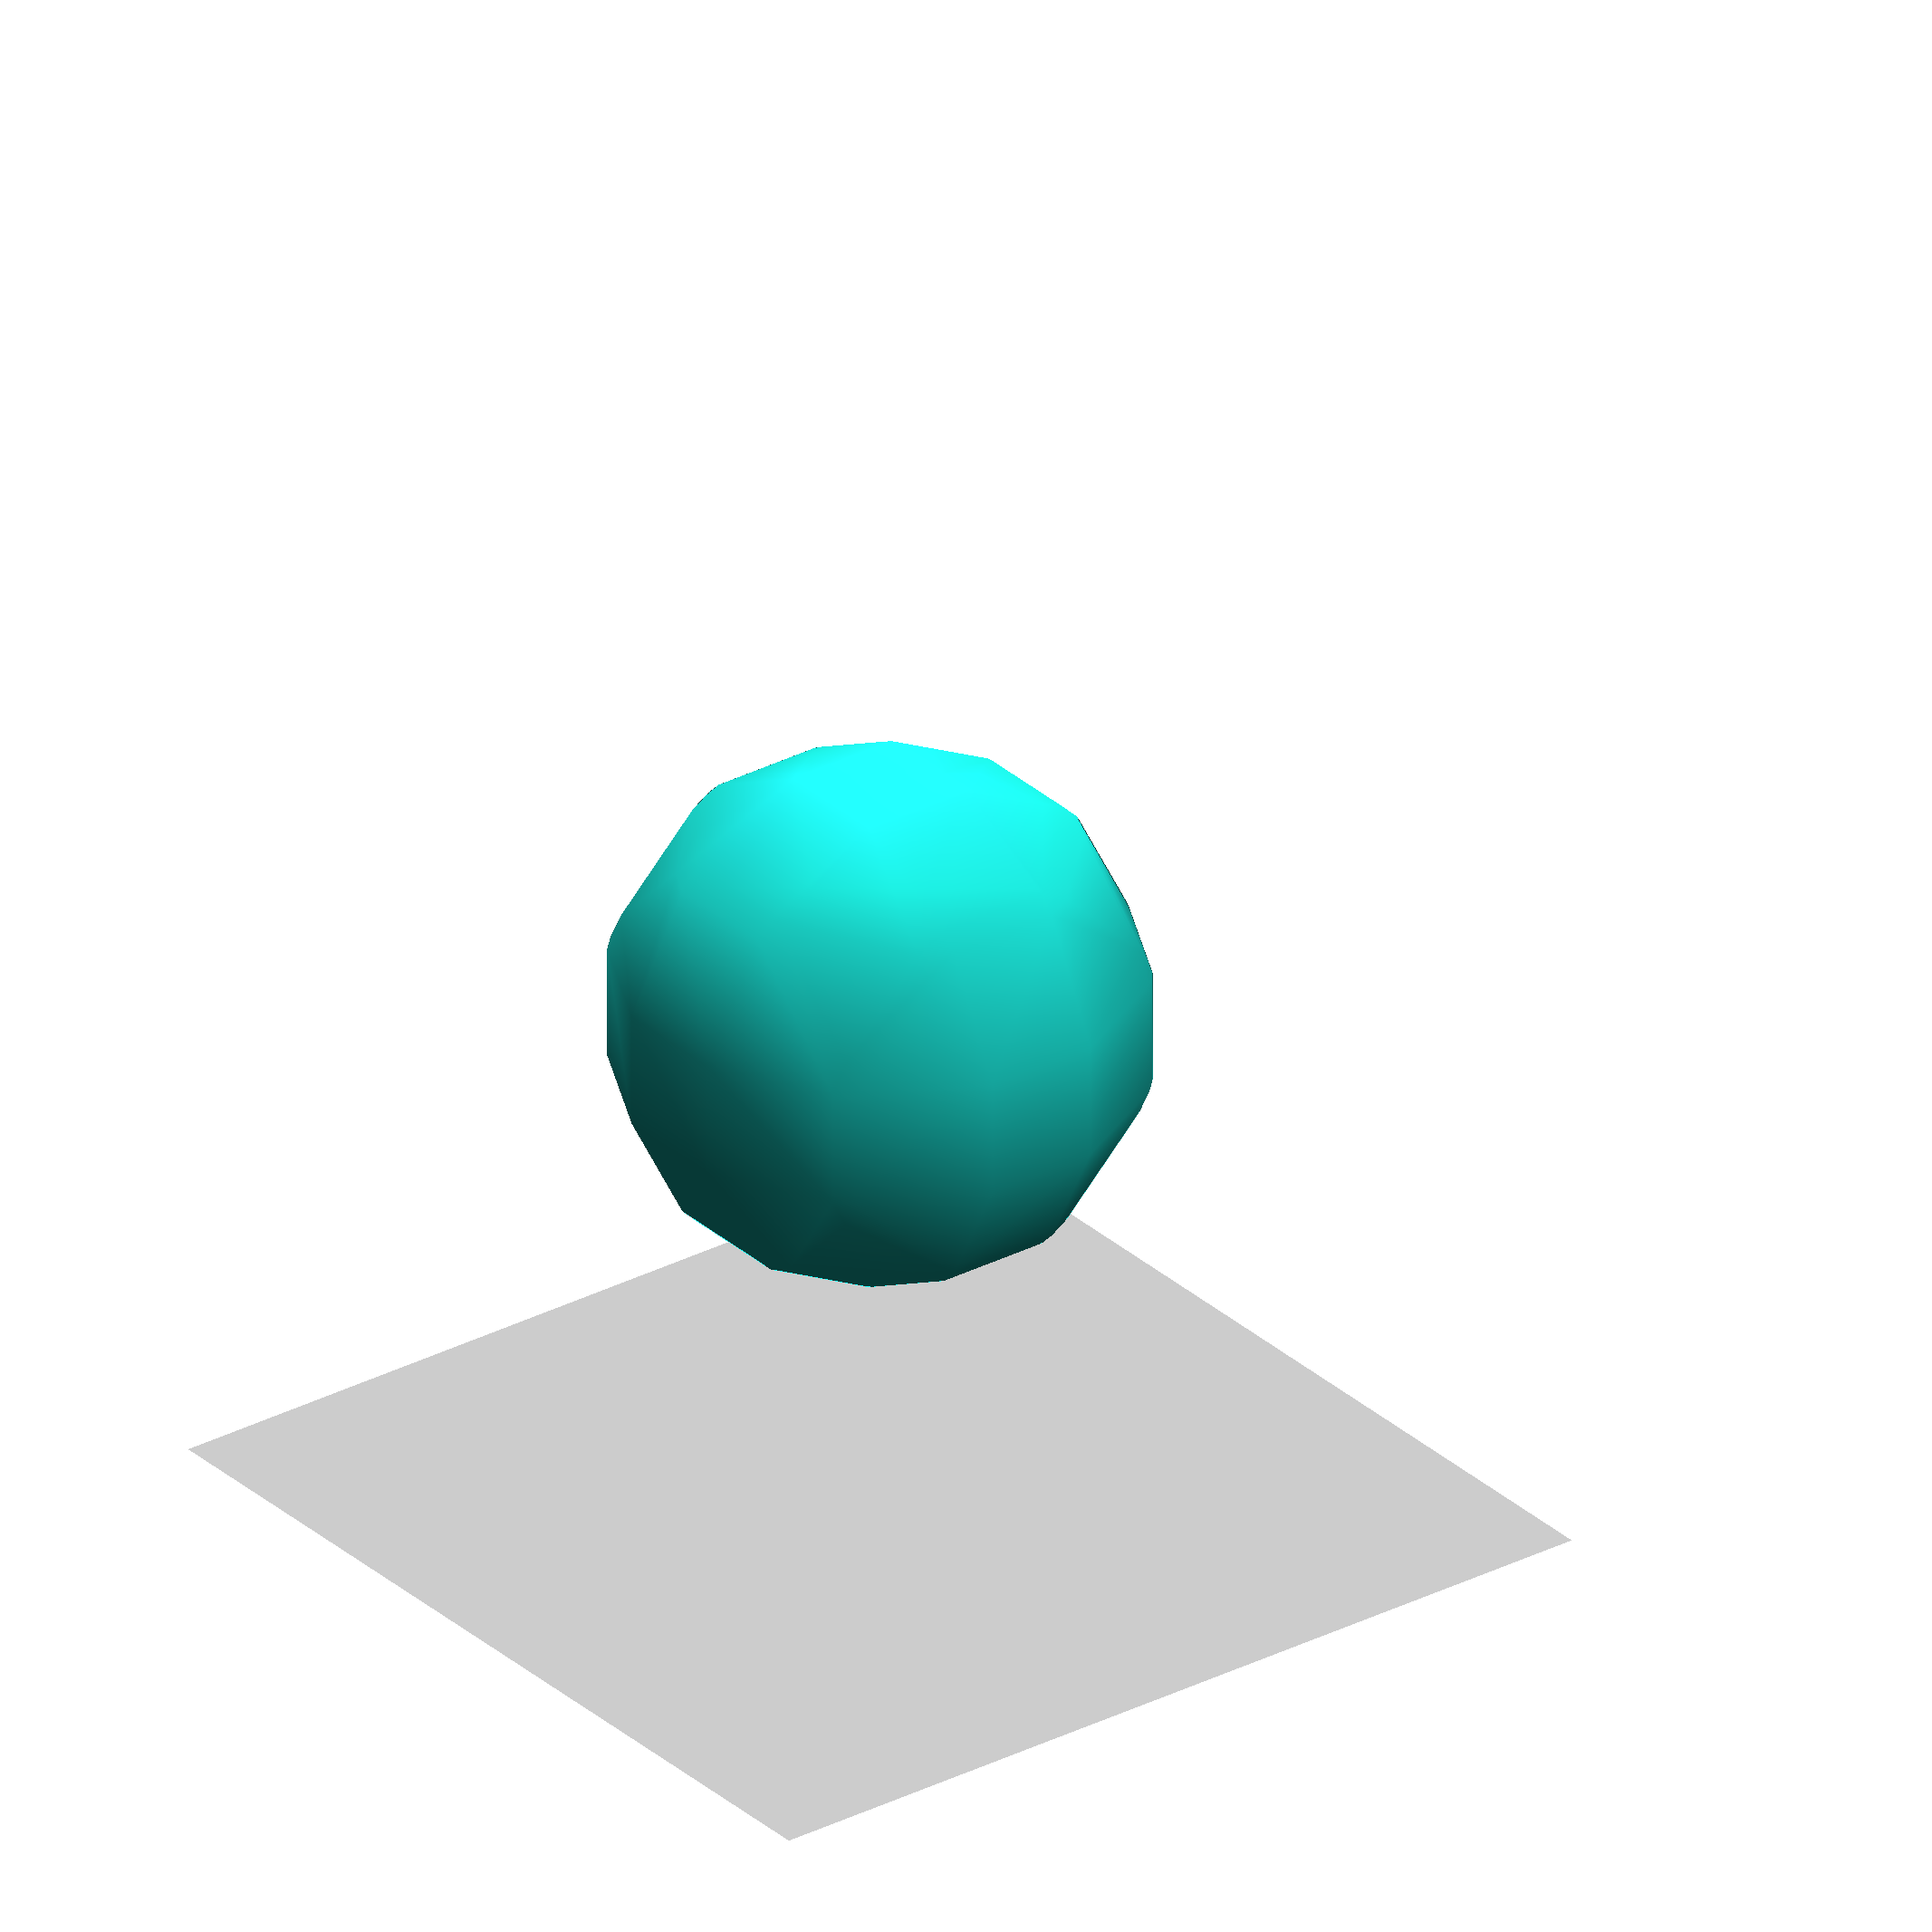
\includegraphics[width=0.18\linewidth]{chapter_background/img/real_8x8x8.png} &
    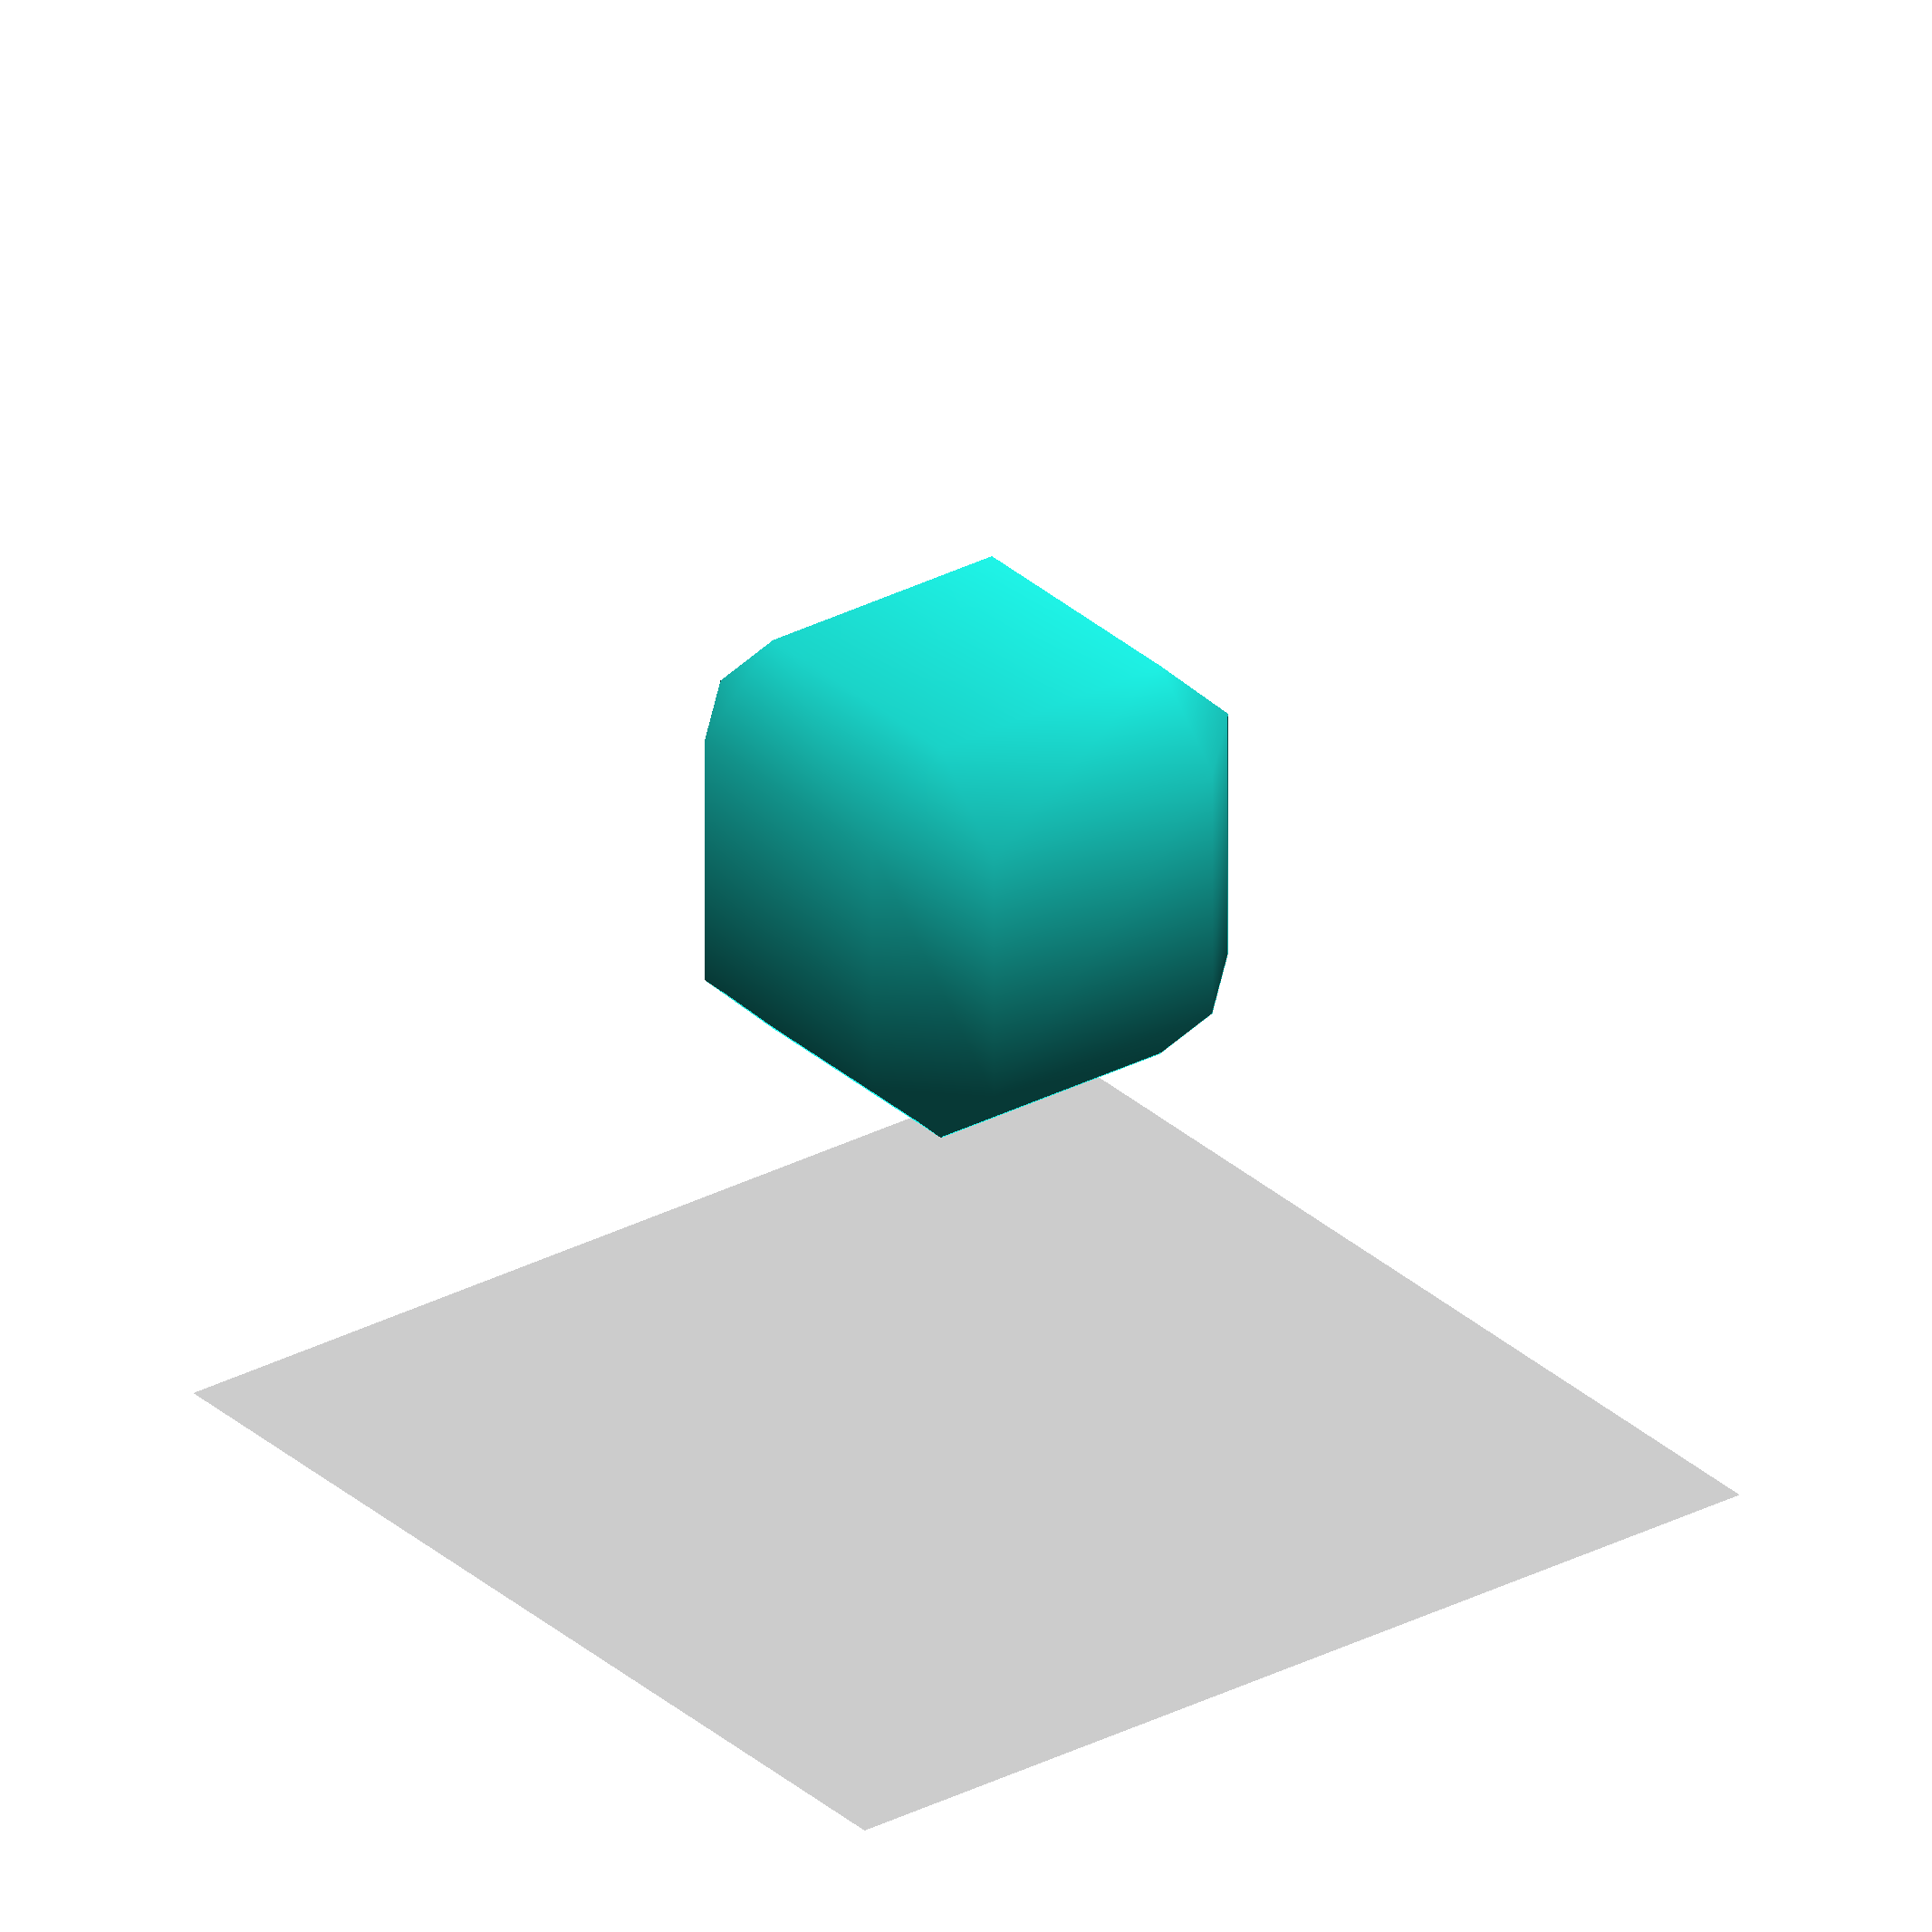
\includegraphics[width=0.18\linewidth]{chapter_background/img/real_4x4x4.png}
    \\
    Binary & Real & Real & Real & Real \\
    $32^3$ & $32^3$ & $16^3$ & $8^3$ & $4^3$ \\
  \end{tabular}
  \caption[Volumetric antialiasing at different resolutions]{A
    volumetric sphere, with and without antialiasing, at several
    different resolutions.}
  \label{fig:background:volquality}
\end{figure}

\subsection{Voxelisation}

The process of transforming a mesh into a volumetric structure is
referred to as voxelisation. Intuitively, this voxelisation process
discretises the mesh. It is no longer possible to reproduce a
non-integer form of the original mesh - a surface noticeably
constructed out of small cubes. Ideally, there should be minimal
visual degradation between viewing the original mesh and the voxelised
object.  Just as anti-aliasing is possible in 2D graphics, it is also
possible with 3D volumes. This is achieved by using real numbers
inside a voxel, instead of just a binary value.  This results in very
low distortion, provided the resolution is sensibly selected. This is
shown in Figure~\ref{fig:background:volquality}, the sphere encoded
using binary values is clearly built out of cubes, where as even a
small real value volume remains representative.

Generating a 2D image from 2D vector graphics (such as polygons) is
called rasterisation. This involves tracing a ray while counting the
number of line intersections. If the count is odd, colour in pixel and
move onto the next. If the count is even, just move onto the next
pixel. Voxelisation follows a similar idea, except it is performed in
three dimensions instead of two. This is done by tracing rays through
the X, Y and Z planes separately to produce three separate
volumes. These volumes are then combined in some way, typically by
ensuring each XYZ coordinate has been set in at least two volumes. We
show this visually in Figure~\ref{fig:background:voltracing}, where
error has been introduced by only voxelising the Stanford
Bunny\footnote{http://graphics.stanford.edu/data/3Dscanrep} from a
single direction.

\begin{figure}
  \centering
  \begin{tabular}{ccccc}
    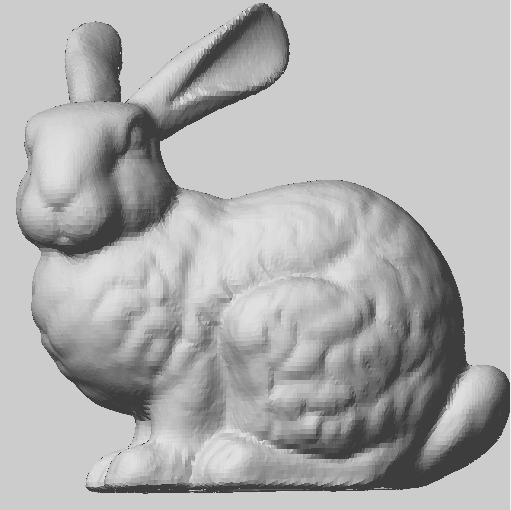
\includegraphics[width=0.17\linewidth]{imggen/vox_xyz/bunny_original.png} &
    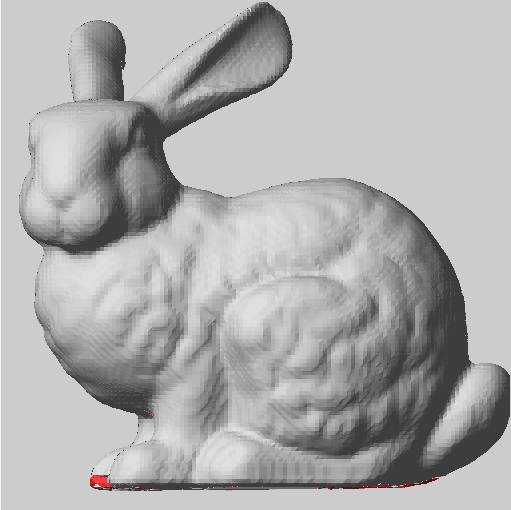
\includegraphics[width=0.17\linewidth]{imggen/vox_xyz/bunny_voxX.png} &
    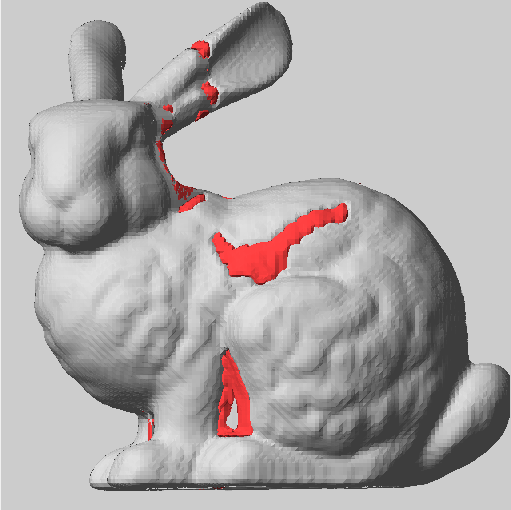
\includegraphics[width=0.17\linewidth]{imggen/vox_xyz/bunny_voxY.png} &
    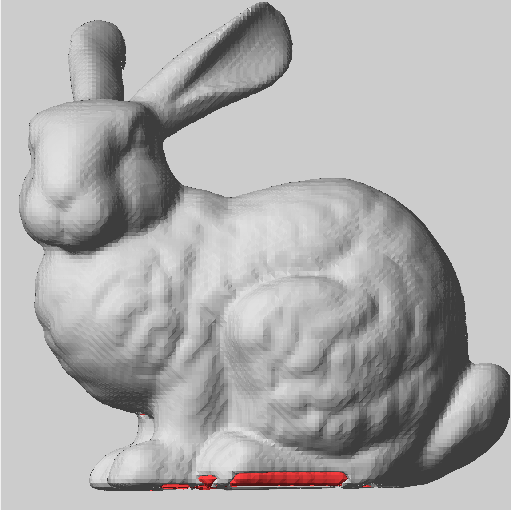
\includegraphics[width=0.17\linewidth]{imggen/vox_xyz/bunny_voxZ.png} &
    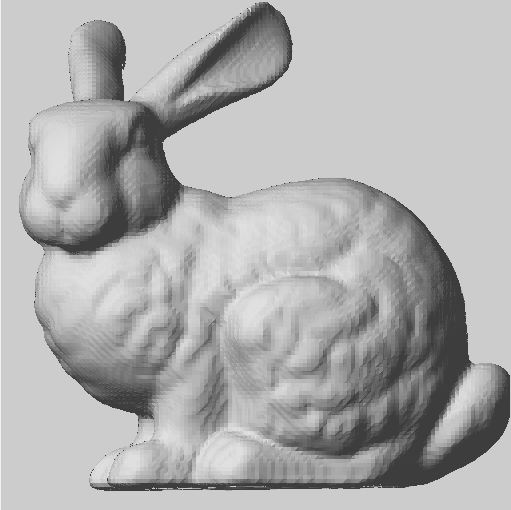
\includegraphics[width=0.17\linewidth]{imggen/vox_xyz/bunny_voxXYZ.png} \\
    Original & Voxelised & Voxelised & Voxelised & Voxelised \\
    Mesh     & Traced X  & Traced Y  & Traced Z  & Traced XYZ \\
  \end{tabular}
  \caption[Voxelisation error due to limiting ray tracing
  directions]{Voxelised results of the Stanford Bunny (original shown
    on left). The first three volumes have been voxelised by tracing
    from either X, Y or Z directions. The final volume (right most) is
    generated by voting. Red patches fill in voxels which have been
    missed. Each volume is $128^3$ in size.}
  \label{fig:background:voltracing}
\end{figure}

\subsection{Computing an Isosurface}

Perhaps the most popular method for computing the isosurface of a
volume is Marching Cubes~\cite{lorensen1987marching}, developed in
1987. The algorithm traverses through all voxels, using the value of
eight neighbouring voxels to form eight binary values, a single
byte. This byte can be used to lookup a known polygon configuration
from a table of $2^8 = 256$ entries. However, in the first version of
Marching Cubes, only 15 unique polygon configurations were
stored. This lead to cases of ambiguity when looking up the
meshes. The side effect of this is that meshes would sometimes end up
having holes in them. In~\cite{chernyaev1995marching}, additional
unique configurations were proposed, leading to a total of 33. This
removes the ambiguity, and results in the meshes being closed or
\textit{water tight}.


\subsection{Size, Compression and Formats}
\label{sec:background:volstorage}

There are many more factors which have to be considered when working
with volumetric representations of objects, as opposed to a standard
mesh.

To start with, the \textbf{size} of the volume (in terms of bytes)
grows much more rapidly than it would in a 2D image. In order to
represent a sensible amount of depth in a $128 \times 128$ image, a
volume of $128^3$ voxels is likely needed. If this is uncompressed and
encoded as bytes, it will require 2MB of storage. Scale this up to a
dataset of maybe 50,000 samples, use a slightly larger volume, and it
is clear that this may begin to cause problems.

One solution might be to compress the volumes. However, compression
introduces a significant computational overhead. It is a common trade
off between processing power, available storage and I/O speeds. While
compression of images has come away (even JPEG decoding is hardware
accelerated on some platforms now), the same is not true for 3D
volumes. Compression options are of course available (Run Length
Encoding, Huffman Coding and LZ77, just to name a few), but the on
large volumes being read many times per second, the CPU could easily
become the bottleneck.

File formats is another important consideration. There are many
formats for storing volumetric data. Typically, these formats have
been developed for the medical field for use with MRI, CT scans and
the like. As such, these formats often include space for details such
as patient information, along with a metadata describing the
resolution and bit depth of the volumetric data. An argument can be
made that none of this information is required if the volumetric
representation is used as an intermediary state and doesn't have to be
processed by \textit{humans}. This applies to the work presented in
this thesis. The volumetric representation used in the work described
throughout this thesis is a contiguous array of bytes, which can be
very efficiently read into memory.


\section{Related Work}

% Throughout this thesis, each chapter will have its own section
% discussing related work. However, this section serves to briefly
% mention a few of the most significant works which has strongly
% influenced general ideas described in this thesis. There is one
% caveat; it can be argued that perhaps the most influential idea in
% this work is convolutional neural networks. However, use of CNNs has
% become so ubiquitous and accepted that a literature review on this
% topic is certainly out of the scope of this thesis.

% Long proposed the idea of a fully convolutional network
% in~\cite{long2015fully} for the purpose of refined semantic
% segmentation of images. More concretely, their proposed architecture
% has no fully connected layers involved in this network which enables
% input to have varying resolution. Instead, it reshapes the original
% fully connected layer into a $1 \times 1$ convolution, allowing the
% network to be fined tuned from ImageNet~\cite{krizhevsky2012imagenet}
% classification.

This section attempts to provide a comprehensive literature review of
the works relevant to this thesis. This thesis focuses primarily on
the 3D reconstruction of human faces and bodies. Much of the
literature discussed in this chapter has an obvious
relevance. However, in the cases which are less obvious, connections
have attempted to be made with references to the relevant chapter
and section.


\subsection{Depth Estimation}

\subsection{Shape from Shading}

\subsection{Morphable Model Fitting}

\subsection{Semantic Segmentation}

Semantic segmentation is the process by which pixels of an image are
labelled by the objects contained in the image. For example, all dogs
may be labelled as red, while cats may be labelled as green. In order
for this to work, context is required, both locally and
globally. Global context tells us what is in the image and roughly
where a particular object may be located. Local context then refines
this global information, defining boundaries between classes with much
greater precision.

Classical approaches to semantic segmentation involved first
segmenting the image using statistical models, followed by
individually classifying the segmented objects. See for
example~\cite{arbelaez2012semantic,carreira2012semantic}, which use a
Conditional Random Field to separate the image. However, these methods
generally struggle to adequately incorporate high and low level
feature descriptors necessary for high quality segmentation.

CNNs drastically changed the landscape of semantic segmentation. The
first work producing satisfactory quality semantic segmentation was
the Fully Convolutional Network (FCN) described
in~\cite{long2015fully}, which was based on
VGG-16~\cite{simonyan2014vgg}. In this work, information is forked
from different layers throughout the network. Each fork is used to
produce an intensity map for all known class (initially 59, from the
PASCAL VOC 2010 dataset~\cite{everingham2010pascal}). Forks earlier on
in the network provide very detailed but noisy predictions about the
location of classes, where as the latter forks are have very little
noise, but can only approximate the location of a class. A diagram of
the structure of FCN is shown in Figure~\ref{fig:background:fcn}. FCN
was not intended to be trained from scratch. Instead, training was
initialised from the parameters of VGG-16, once the network had been
trained on the ImageNet dataset~\cite{krizhevsky2012imagenet} for the
task of classification. The parameters in the latter layers of the
network were reshaped from linear layers into a $1\times 1$
convolution. An interesting side effect of which, is the ability for
the network to accept inputs of arbitrary sizes. The size of the input
no longer dictates the number of parameters in the linear layers. Due
to its simplicity and (at the time) \textit{state of the art} results,
it is no surprise the ideas behind FCN have become to standard for
modern semantic segmentation methods.

Still, one of the limitations of FCN is that the resolution of its
predictions are quite low. As such, several methods have proposed
extensions to FCN to compensate for this limitation. The most common
addition has been to add a CRF to the output of the network, to
provide further refinement. The work of \cite{chen2015semantic}
first upsamples the predicted scores using bilinear interpolation
and then refines the output by applying a dense CRF. The method of
\cite{zheng2015conditional} performs recurrent end-to-end training of
the FCN and the dense CRF. Finally, the work in \cite{noh2015learning}
employs learnt deconvolution layers, as opposed to fixing the
parameters with an interpolation filter (as in FCN). These filters
learn to reconstruct the object's shape, in addition to upsampling its
input.

In the past year or so, the Encoder-Decode network architecture has
gained a great deal of popularity. This architecture network reduces
the spatial dimensionality as they pass through the
\textit{encoder}. These features are then upsampled again using a
\textit{decoder} part of the network, while being recombined with
lower level information, much like in FCN~\cite{long2015fully}. This
architecture has also been referred to as an hourglass network. This
name was first used in~\cite{newell2016stacked}, and performed human
pose estimation with great precision. This level of precision is due
to the being suited to combining features from the high and low parts
of the network efficiently (i.e. combining both global and local
context). As such, similar architectures have been used for semantic
segmentation problems. For example,
SegNet~\cite{badrinarayanan2017segnet} uses an Encoder-Decoder
architecture is used to perform semantic segmentation on 11 classes
for autonomous driving in real time.

Architectures aside, a main drawback of this supervised approach to
semantic segmentation is producing large quantities of detailed
groundtruth semantic masks. There are several large datasets already
available, such as PASCAL VOC~\cite{everingham2010pascal}, Microsoft
COCO~\cite{lin2014microsoft} and
Cityscapes~\cite{cordts2016cityscapes}. All of these datasets are
fairly constrained in terms of the number of known
classes. Respectively, these datasets have 59, 183 and 30 known
classes. This is problematic when it comes to making semantic
segmentation a viable tool for general semantic segmentation
\textit{in-the-wild}. As such, numerous approaches have been devised
to train these models in ways requiring less human
intervention. In~\cite{richter2016playing}, hooks are added to
visually detailed computer games, to allow automatic generation of
instance aware semantic segmentation masks. A drawback of this is that
most games are far from realistic enough to work on real images. As
such, models trained on this data will also require domain adaptation
- which is an entire research area in itself. In~\cite{bearman2016s},
a weakly supervised approach is presented, where groundtruth semantic
segmentation masks are avoided entirely. Instead, the method learns
the semantic segmentation task from just a single point on each
object.

Another approach is described in~\cite{hu2018learning}, where the
training set is formed of images where all classes are annotated with
bounding boxes. However, only some classes have groundtruth masks. The
network is trained to produce both bounding boxes and semantic
segmentation masks simultaneously by learning a mapping between the
visual embedding from the bounding box feature extractors, to the
semantic segmentation feature extractors. The paper describes this
working on 3000 segmentation classes. They refer to this approach as
\textit{partially} supervised, as some groundtruth data is
required. Additionally, the method has been shown to be able to
segment up to 3000 classes - far higher than~\cite{long2015fully},
which was trained on the 59 classes from VOC PASCAL
2010~\cite{everingham2010pascal}.

The primary focus of this thesis is not on semantic
segmentation. However, in Chapter~\ref{chapter:seg}, we describe our
facial part segmentation. However, deep learning based approaches to semantic
segmentation, particularly the fully convolutional approach in
~\cite{long2015fully}, have had a strong influence on how we approach
the problems of 3D reconstruction.

%



\begin{figure}
  \centering
  \begin{tikzpicture}[scale=0.9]
  \networkLayer{3.0}{0.48}{0}{0.0}{color=green!30}{96}
  \networkLayer{1.5}{1.28}{0.48}{0.0}{color=green!30}{256}
  \networkLayer{0.75}{1.92}{1.76}{0.0}{color=green!30}{384}
  \networkLayer{0.75}{1.92}{3.68}{0.0}{color=green!30}{384}
  \networkLayer{0.75}{1.28}{5.60}{0.0}{color=green!30}{256}
  \networkLayer{0.37}{2.05}{6.88}{0.0}{color=green!30}{4096}
  \networkLayer{0.37}{2.05}{8.93}{0.0}{color=green!30}{4096}
  \networkLayer{0.37}{0.5}{10.98}{0.0}{color=green!30}{1000}

  \networkLayer{0.75}{0.5}{12}{0.0}{color=red!30}{$\times 2$}
  \networkLayer{1.5}{0.5}{13}{0.0}{color=red!30}{$\times 2$}
  \networkLayer{3}{0.5}{14.5}{0.0}{color=red!30}{$\times 2$}

  \draw [>->] (1.92,1.75) -- (1.92,2.5) -- (13.5,2.5);
  \draw [>->] (6.88,1) -- (6.88,1.25) -- (12.5,1.25);

  \draw (13.5,3) circle [radius=0.3] node {$+$};
  \draw (12.5,1.75) circle [radius=0.3] node {$+$};
\end{tikzpicture}
\caption[The VGG-16 network]{Basic VGG-16~\cite{simonyan2014vgg}
  network with modifications added from
  FCN~\cite{long2015fully}. Information from lower levels of the
  network summed to upsampled output of the tailing end of the
  network. The number of features is shown below each convolution.}
\label{fig:background:fcn}
\end{figure}











%%% Local Variables:
%%% TeX-master: "../thesis"
%%% End:
